\documentclass[tikz]{standalone}

\begin{document}

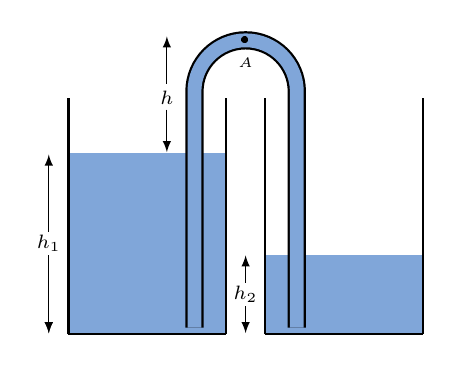
\begin{tikzpicture}
    \fill[blue!70!green!50] (0,0) rectangle (2,2.3);
    \draw[thick] (0,0)-- (2,0);
    \draw[thick] (0,0)-- (0,3);
    \draw[thick] (2,0)-- (2,3);
    \fill[blue!70!green!50] (2.5,0) rectangle ++(2,1);
    \draw[thick] (2.5,0)-- (4.5,0);
    \draw[thick] (2.5,0)-- (2.5,3);
    \draw[thick] (4.5,0)-- (4.5,3);
    \draw[thick,double=blue!70!green!50,double distance=5pt,draw=black] (1.6,0.08)-- +(0,3) arc (180:0:0.65) node[midway,label={[shift={(0,-0.65)}]\tiny{$A$}}] {\tiny{\textbullet}}-- +(0,-3);
    \draw [latex-] (-0.25,2.28)--(-0.25,1.3) node [label={[shift={(0,-0.5)}]$\scriptstyle{h_1}$}] {};
    \draw [-latex] (-0.25,1)--(-0.25,0.01);
    \draw [latex-] (2.25,1)--(2.25,0.65) node [label={[shift={(0,-0.5)}]$\scriptstyle{h_2}$}] {};
    \draw [-latex] (2.25,0.35)--(2.25,0.01);
    \draw [-latex] (-0.25,1)--(-0.25,0.01);
    \draw [latex-] (1.25,3.78)--(1.25,3.17) node [label={[shift={(0,-0.5)}]$\scriptstyle{h}$}] {};
    \draw [-latex] (1.25,2.85)--(1.25,2.31);
\end{tikzpicture}

\end{document}